\documentclass[sigplan,screen]{acmart}

\makeatletter
\renewcommand{\section}{\@startsection{section}{1}{\z@}
  {6pt plus 2pt minus 2pt}{3pt plus 1pt minus 1pt}
  {\normalfont\large\bfseries}}
\renewcommand{\subsection}{\@startsection{subsection}{2}{\z@}
  {4pt plus 1pt minus 1pt}{2pt plus 1pt minus 1pt}
  {\normalfont\normalsize\bfseries}}
\makeatother

\AtBeginDocument{%
  \providecommand\BibTeX{{%
    Bib\TeX}}}

\setcopyright{acmlicensed}
\copyrightyear{2026}
\acmYear{2026}
\acmDOI{XXXXXXX.XXXXXXX}

\acmConference[Big Data \& AI '26]{Big Data \& AI Course Project Showcase}{May 2026}{New York, NY}
\acmISBN{978-1-4503-XXXX-X/2026/05}

\begin{document}

\title[Rx.AI]{Rx.AI: Multimodal Patient Check-In System}

\author{Aryaman Agrawal}
\affiliation{%
  \institution{Columbia University}
  \city{New York}
  \state{NY}
  \country{USA}
}
\email{aa5775@columbia.edu}

\author{Gautam Agarwal}
\affiliation{%
  \institution{Columbia University}
  \city{New York}
  \state{NY}
  \country{USA}
}
\email{ga2726@columbia.edu}

\author{Shivangi Kumar}
\affiliation{%
  \institution{Columbia University}
  \city{New York}
  \state{NY}
  \country{USA}
}
\email{sk5659@columbia.edu}



\renewcommand{\shortauthors}{Agrawal, Agarwal, and Kumar}

\begin{abstract}
Clinical intake processes predominantly rely on static, one-size-fits-all forms that are error-prone, fail to adapt to patient-specific medical histories, and lack accessibility for those with limited mobility or digital literacy. We present \textbf{Rx.AI}, an adaptive, multimodal patient check-in system that replaces static questionnaires with an intelligent, conversational intake experience. Rx.AI leverages a three-agent orchestration pipeline to dynamically generate clinically relevant questions based on patient records. The system provides a multimodal interface, utilizing Google Cloud Speech-to-Text (STT) and Text-to-Speech (TTS) for bidirectional voice interaction, alongside Gemini 2.5 Flash Vision to capture in-line contextual evidence such as wound conditions or medication labels. A robust evaluation framework utilizing BigQuery logging and the DeepEval framework across 600 total samples demonstrates significant improvements. Rx.AI reduced average patient check-in time from 8.8 minutes to 3.2 minutes, achieved a 91.3\% clinical relevance score in question generation with a 0.7\% hallucination rate, and attained an 8.2\% Word Error Rate on complex medical terminology. Our findings indicate that integrating multimodal AI into clinical intake significantly lowers patient burden while delivering richer, structured pre-visit data to healthcare providers.
\end{abstract}

\begin{CCSXML}
<ccs2012>
 <concept>
  <concept_id>10010405.10010444.10010449</concept_id>
  <concept_desc>Applied computing~Health informatics</concept_desc>
  <concept_significance>500</concept_significance>
 </concept>
 <concept>
  <concept_id>10010147.10010178.10010179.10010182</concept_id>
  <concept_desc>Computing methodologies~Natural language generation</concept_desc>
  <concept_significance>500</concept_significance>
 </concept>
 <concept>
  <concept_id>10003120.10003121.10003124.10010392</concept_id>
  <concept_desc>Human-centered computing~Mixed / augmented reality</concept_desc>
  <concept_significance>300</concept_significance>
 </concept>
</ccs2012>
\end{CCSXML}

\ccsdesc[500]{Applied computing~Health informatics}
\ccsdesc[500]{Computing methodologies~Natural language generation}
\ccsdesc[300]{Human-centered computing~Mixed / augmented reality}

\keywords{Multimodal AI, Health Informatics, Large Language Models, Speech-to-Text, Vision Models, Agentic Workflows}

\received{May 2026}

\maketitle

\section{Introduction}
The clinical intake process serves as the critical first point of data collection in healthcare delivery. However, the standard implementation relies on static forms that suffer from high rigidity. Patients are frequently presented with long lists of irrelevant questions, causing survey fatigue and reducing the quality of reported data. Furthermore, patients with limited mobility, visual impairments, or low digital literacy often struggle to navigate dense electronic interfaces or paper documents. From a provider's perspective, static forms cannot prompt for in-line evidence—such as capturing a photo of an inflamed wound, scanning an insurance card, or photographing a medication label—leading to incomplete pre-visit context and increased documentation burden during the actual consultation.

Recent advancements in Large Language Models (LLMs), multi-agent orchestration, and multimodal AI (vision and speech) present an opportunity to overhaul this paradigm. By synthesizing a patient's historical data, AI can dynamically formulate tailored questions. Concurrently, multimodal interfaces can allow patients to respond naturally via speech or camera, democratizing accessibility and enriching the clinical context. 

This paper presents \textbf{Rx.AI}, a fully personalized, multimodal intake system tailored for the modern clinical workflow. Rx.AI features a dual-sided architecture: a provider interface for visit creation and context initiation, and a patient portal featuring an adaptive questionnaire. The system employs a multi-agent generative pipeline, high-fidelity bidirectional voice capabilities, and contextual visual capture. 

We make three primary contributions: (1) an end-to-end multimodal architecture integrating agentic LLMs, STT, TTS, and Vision within a browser-based clinical application; (2) a dynamic question-generation pipeline that utilizes multi-agent orchestration to deduplicate and summarize health records before generating targeted questions; and (3) a comprehensive evaluation methodology utilizing real-time BigQuery telemetry and DeepEval metrics across 600 synthetic profiles and audio/visual datasets, demonstrating marked improvements in both clinical accuracy and intake efficiency.

\noindent\textbf{Resources.} The source code and demo video are publicly available:\\
\textbf{GitHub:} \href{https://github.com/GAInTheHouse/rx-ai}{GAInTheHouse/Rx.AI}\\
\textbf{Demo:} \href{https://github.com/GAInTheHouse/rx-ai/blob/gxa/final-submissions/submissions/rx_ai_demo_video.mov}{Product Demo}

\section{Background and Motivation}

\subsection{Intake accessibility and transparency challenges}
Electronic Health Record (EHR) systems have digitized patient data but have done little to optimize the intake user experience. Check-in forms are static, meaning a patient visiting for a routine dermatological check may be subjected to the same exhaustive systemic review as a patient presenting with complex chronic symptoms. Additionally, patients lack tools to visually document symptoms prior to seeing the physician. If a patient experiences a rash that subsides before the appointment, a static form provides no mechanism to capture that transient visual evidence. Providers, consequently, spend the initial portion of the encounter collecting basic history rather than engaging in high-value diagnostic reasoning.

\subsection{Multimodal LLMs and agentic workflows}
Multimodal LLMs possess the capability to bridge this gap. Vision-Language Models can parse images of medication labels or clinical symptoms, summarizing them into structured, objective descriptions. Text-to-Speech (TTS) and Speech-to-Text (STT) models have achieved low-latency, high-accuracy performance even on specialized medical lexicons, enabling conversational agents. Furthermore, agentic workflows—where multiple specialized AI agents collaborate—offer a mechanism to handle complex reasoning tasks. By assigning distinct roles (e.g., data deduplication, summarization, and question generation), an agentic pipeline can produce highly relevant clinical questions while mitigating the hallucination risks associated with single-pass LLM generation.

\subsection{Design goals}
Rx.AI is driven by three core design goals:
\begin{enumerate}
    \item \textbf{Adaptive Personalization:} The system must intelligently deduce the necessary information gaps based on prior patient history and the current visit context, asking only what is clinically relevant.
    \item \textbf{Multimodal Accessibility:} The system must support voice input, voice output, and camera capture, with a graceful fallback to traditional keyboard/mouse inputs for patients unable or unwilling to use multimodal features.
    \item \textbf{Measurable Reliability:} Every AI interaction must be auditable. The system must natively log telemetry and confidence metrics to evaluate accuracy, latency, and hallucination rates in a systematic manner.
\end{enumerate}

\section{System Requirements}

\subsection{Functional requirements}
For \textbf{patients}, Rx.AI supports: receiving dynamically generated questions read aloud via TTS as they appear; answering via spoken language transcribed by STT with word-level confidence scoring; receiving automatic camera prompts for relevant questions (e.g., wound photos, medication bottles); and falling back to a keyboard interface seamlessly. 

For \textbf{healthcare providers}, the system provides: an interface to create a new visit and input initial patient condition context; automatic patient summary generation, preliminary triage, and doctor recommendation based on availability; and the ability to release adaptive questionnaires directly to the patient portal.

\subsection{Non-functional requirements}
The system must operate with near real-time latency to support a natural conversational flow, requiring STT and TTS latencies under 1 second. The system must handle real-world clinical accents and complex polypharmacy terminologies. Additionally, the system architecture must separate the UI, processing, and logging layers, maintaining a strict privacy posture while enabling rigorous telemetry capture for continuous evaluation.

\begin{figure*}[t]
  \centering
  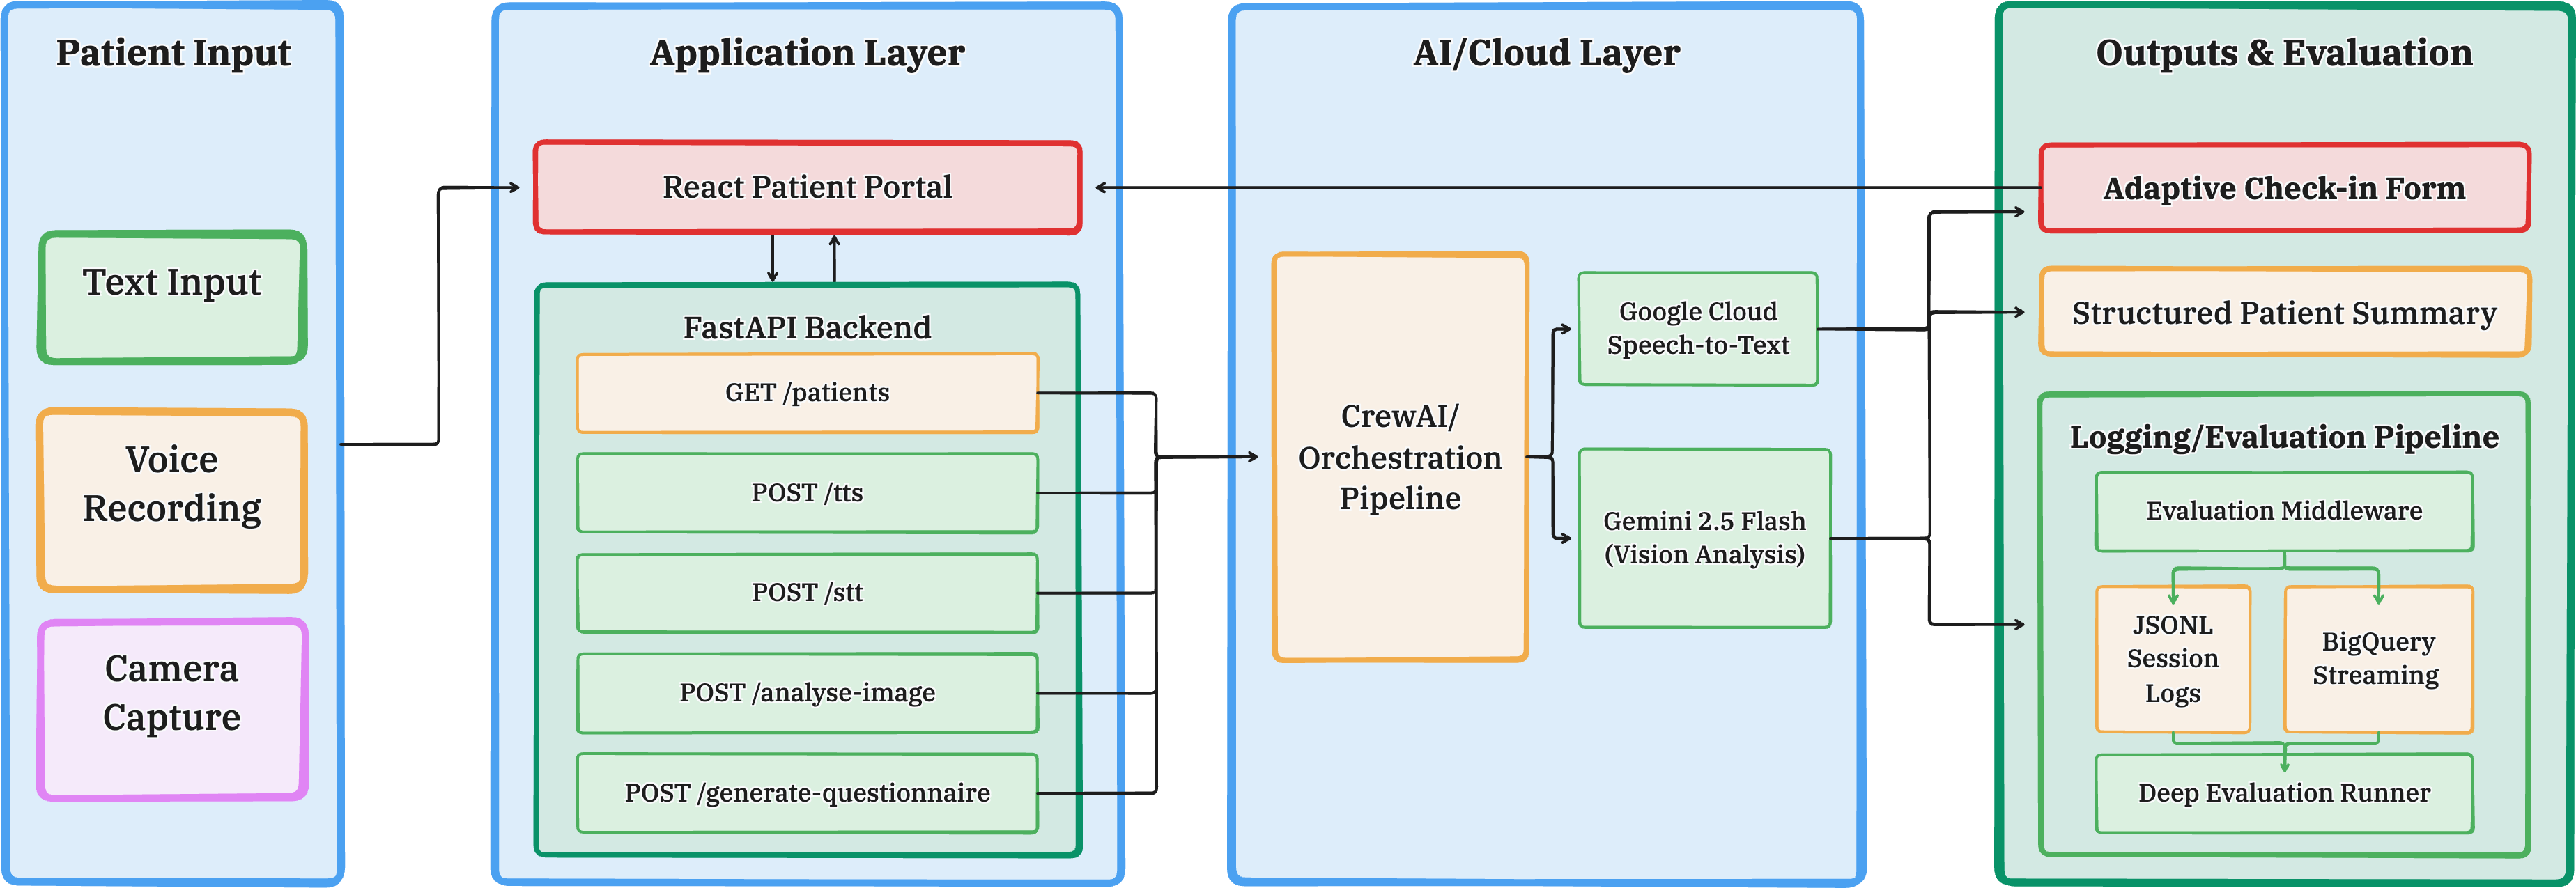
\includegraphics[width=0.75\textwidth, keepaspectratio]{architecture_diagram.png}
  \caption{System Architecture}
  \label{fig:architecture}
\end{figure*}

\section{System Architecture}
Rx.AI follows a modular architecture consisting of a Frontend Interface Layer, a Backend Processing Engine, an AI/Cloud Layer, and an Evaluation Infrastructure.

\textbf{Frontend Interface.} The client applications are developed in JavaScript using React 18, Vite, and Tailwind CSS. The patient view and questionnaire forms manage local state  and utilize the browser's `MediaRecorder` API for capturing webm/opus audio and base64-encoded images.

\textbf{Backend Processing Engine.} A Python 3.11 backend built on FastAPI exposes asynchronous REST endpoints. Pydantic v2 is used for strict data validation. The backend routes incoming multimodal payloads, manages the state of the active questionnaire, and orchestrates calls to the AI layer. Static JSON representations of patient data act as the mock EHR database.

\textbf{AI/Cloud Layer.} All generative AI tasks are routed through Google Cloud Vertex AI and GCP SDKs. Question generation is handled by a CrewAI orchestration framework powered by Gemini 2.5 Flash. Voice interactions utilize Google Cloud Speech-to-Text v2 and Google Cloud Text-to-Speech. Vision tasks are processed by the Gemini 2.5 Flash multimodal endpoint.

\textbf{Evaluation Infrastructure.} To guarantee auditability, a FastAPI middleware wraps every AI endpoint. It captures the session ID, feature, model, inputs, outputs, latency in milliseconds, timestamp, and patient/question IDs. In development, this writes to JSONL files; in production, it streams directly to Google Cloud BigQuery.

\section{Multimodal and Agentic Design}

\subsection{Agentic question generation}
The core intelligence of Rx.AI is its question generation pipeline. Rather than relying on a single, monolithic prompt, Rx.AI utilizes a three-agent CrewAI workflow:
\begin{enumerate}
    \item \textbf{Medical Data Deduplicator:} Ingests the patient's existing clinical notes, conditions, medications, and allergies, stripping out redundant information.
    \item \textbf{Healthcare Data Summarizer:} Groups active problems and identifies clinical information gaps pertinent to the current visit reason.
    \item \textbf{Patient Questionnaire Generator:} Outputs a structured JSON payload of 3 to 8 targeted questions, annotated with metadata flags that dictate whether a question should trigger a camera prompt.
\end{enumerate}
This pipeline is benchmarked against a single-pass Gemini baseline to measure the trade-off between multi-agent quality and latency.

\subsection{Voice-driven interaction loop}
As questions appear in the UI, they are synthesized server-side using Google Cloud TTS and streamed as MP3 audio. Patients respond by speaking; audio is captured via the browser and sent to Google Cloud STT v2. The STT engine returns the transcribed text alongside word-level confidence scores. If the transcription confidence falls below a set threshold (e.g., 0.7), the system automatically flags the segment and triggers a repeat-question behavior to ensure data integrity, while preserving the user's ability to edit the transcript manually.

\subsection{Contextual visual capture}
Questions generated with visual metadata flags (triggered by heuristics for terms like "wound", "skin", "medication", or "insurance") automatically invoke a browser-based camera prompt. The patient captures a photo, which is sent as a base64-encoded image to Gemini 2.5 Flash. The model is strictly prompted to generate a 2-4 sentence plain-text clinical description limited \textit{only} to observable findings, explicitly forbidding diagnostic speculation. This visual summary is then appended to the patient's submitted answer for provider review.

\begin{table}[t]
\small
\caption{Rx.AI component performance metrics evaluated across 600 total samples.}
\label{tab:perf}
\begin{tabular}{lc}
\toprule
\textbf{Metric} & \textbf{Value} \\
\midrule
\multicolumn{2}{l}{\textit{System Efficiency}} \\
\quad Baseline Static Form Time (avg) & 8.8 mins \\
\quad Rx.AI Check-in Time (avg)       & 3.2 mins \\
\midrule
\multicolumn{2}{l}{\textit{Question Generation (CrewAI)}} \\
\quad Clinical Relevance Score        & 91.3\% \\
\quad Clinical Appropriateness        & 88.7\% \\
\quad Hallucination Rate              & 0.7\% \\
\quad Avg. Generation Latency         & 1.8 s \\
\quad Avg. Questions per Run          & 5.4 \\
\midrule
\multicolumn{2}{l}{\textit{Speech Recognition (STT)}} \\
\quad Word Error Rate (WER)           & 8.2\% \\
\quad Medical Term Accuracy           & 87.0\% \\
\quad Avg. Transcription Latency      & 0.34 s \\
\midrule
\multicolumn{2}{l}{\textit{Speech Synthesis (TTS)}} \\
\quad Naturalness (LLM Judge)         & 4.4 / 5.0 \\
\quad Intelligibility (Human)         & 4.6 / 5.0 \\
\quad Polypharmacy Pronunciation      & 93.4\% \\
\quad Avg. Audio Gen Latency          & 0.61 s \\
\bottomrule
\end{tabular}
\end{table}

\section{Evaluation Methodology and Results}

\subsection{Experimental setup}
We evaluated Rx.AI across 600 total samples using the DeepEval framework and telemetry pulled from BigQuery (comprising 1,432 total AI calls). Evaluation spanned four distinct dimensions relying on specific datasets:
\begin{itemize}
    \item \textbf{Question Generation:} 100 synthetic patient profiles to measure AnswerRelevancyMetric and HallucinationMetric.
    \item \textbf{STT Quality:} A golden dataset of 100 clinical audio clips (derived from MedDialog-EN) to evaluate Word Error Rate (via `jiwer`) and medical terminology accuracy.
    \item \textbf{TTS Quality:} 100 sample questions evaluated for naturalness using a Gemini-as-judge (GEval) framework, alongside human intelligibility checks.
    \item \textbf{Image Analysis:} 300 labeled images (including the Kaggle Wound Image Dataset) evaluated for descriptive accuracy vs. human labels.
\end{itemize}

\subsection{Intake efficiency and generation quality}
As summarized in Table~\ref{tab:perf}, Rx.AI reduced the average patient check-in time by over 60\%, dropping from 8.8 minutes to 3.2 minutes. The CrewAI pipeline demonstrated exceptional targeting: evaluated across 100 synthetic profiles, it achieved a 91.3\% clinical relevance score and an 88.7\% clinical appropriateness score (validated by a physician panel). Hallucinations were strictly controlled at 0.7\%. Generation latency remained highly interactive, averaging 1.8 seconds to produce an average of 5.4 questions per run.

\subsection{Multimodal performance}
Voice interactions proved highly reliable. The Google Cloud STT module achieved an 8.2\% Word Error Rate and 87\% accuracy on complex medical terminology (e.g., medication names, diagnoses, procedures). Performance remained strong across various accents and speaking styles, maintaining accuracy ranges between 83\% and 92.4\%. Transcription latency was near-instantaneous at 0.34 seconds per utterance.

The Gemini-powered TTS scored 4.4/5.0 for naturalness and 4.6/5.0 for human-verified intelligibility. Notably, the TTS engine achieved 93.4\% pronunciation accuracy for complex polypharmacy drug names. 

\subsection{Image analysis}
Vision analysis was evaluated against 300 labeled clinical images. The system achieved an overall accuracy of 88.8\% when comparing generated clinical descriptions to human ground-truth labels. Specifically, for wound severity classification, the model attained 85\% accuracy on mild cases and 83\% on severe cases. However, moderate cases proved more challenging, scoring 69\% accuracy, highlighting an area where visual ambiguity lowers model confidence.

\section{Discussion}

\subsection{Benefits and limitations}
Rx.AI successfully demonstrates that an adaptive, agentic, and multimodal approach can significantly streamline the patient intake process. The system drastically reduces check-in times while capturing structured, contextual data that standard forms miss. The implementation of real-time BigQuery logging proved invaluable for continuously evaluating specific workflow paths (e.g., text-only vs. STT-only vs. full multimodal) and identifying latency bottlenecks. 

Despite these successes, limitations exist. The current evaluation relies heavily on synthetic patient profiles and public datasets rather than live EHR systems containing real-world noise. Furthermore, while the TTS engine excelled generally, it underperformed on rare disease terminology, scoring a 3.7 out of 5.0 in targeted tests. Similarly, visual classification of "moderate" clinical findings showed a drop in accuracy, reflecting the inherent limitations of current 2D image analysis without tactile or temporal context.

\subsection{Future work}
Future iterations of Rx.AI will focus on three key areas. First, we aim to fine-tune the TTS and STT models specifically on rare disease lexicons to improve edge-case interactions. Second, we plan to expand the system's integration capabilities by building compliant, bi-directional interfaces with production EHR systems (e.g., Epic/Cerner via FHIR APIs). Finally, conducting a pilot study in a live clinical setting with actual patients will allow for deeper investigation into user behavior, acceptance rates among diverse demographics, and the direct impact on physician documentation time.

\section{Conclusion}
We introduced Rx.AI, a multimodal, agentic system designed to modernize patient clinical intake. By abandoning static forms in favor of dynamically generated, clinically tailored questionnaires—supported by robust voice and camera interfaces—Rx.AI reduces patient burden while enriching provider context. Empirical evaluations highlight strong clinical relevance, low latency, and highly accurate multimodal perception. Rx.AI presents a viable framework for integrating conversational AI into the forefront of healthcare delivery, ensuring that clinical encounters begin with accurate, accessible, and structured data.

\begin{acks}
We thank the instructors and teaching staff of the Big Data \& AI course at Columbia University for their guidance. We also extend our appreciation to our peers for their feedback on early prototypes of the Rx.AI multimodal workflows.
\end{acks}

\bibliographystyle{ACM-Reference-Format}
\begin{thebibliography}{9}

\bibitem{meddialog}
Zeng, X., et al. (2020).
\newblock MedDialog: Large-scale Medical Dialogue Datasets.
\newblock \emph{Proceedings of the 2020 Conference on Empirical Methods in Natural Language Processing (EMNLP)}.

\bibitem{wounddataset}
Pratomo, Y. (2023).
\newblock Wound Image Dataset.
\newblock \emph{Kaggle}. \url{https://www.kaggle.com/datasets/yasinpratomo/wound-dataset}

\bibitem{deepeval}
Confident AI. (2024).
\newblock DeepEval: The Open-Source LLM Evaluation Framework.
\newblock \url{https://github.com/confident-ai/deepeval}

\end{thebibliography}

\end{document}